\documentclass[12pt]{article}
\usepackage[letterpaper,left=16.5mm,right=16.5mm,top=20mm,bottom=20mm,
  headheight=15pt,headsep=7mm,footskip=11mm]{geometry}
\usepackage[T1]{fontenc}
\usepackage[default]{sourcesanspro}
\usepackage{tikz}
\usetikzlibrary{arrows.meta}
\usepackage{fancyhdr}
\pagestyle{fancy}
\fancyhf{}
\renewcommand{\headrulewidth}{0.4pt}
\fancyhead[L]{Week 81 / Buckets of Fish / K\textendash 1}
\fancyfoot[L]{\small Bellingham Math Circle / Week 81 / W81-K-v1}
\fancyfoot[R]{\small \thepage}
\setlength{\parindent}{0pt}
\setlength{\parskip}{0pt}
\linespread{1.12}
\frenchspacing
\raggedright
\tikzset{
  bucket/.style={line width=0.7pt, rounded corners=1.6mm},
  store/.style={line width=0.7pt},
  ans/.style={line width=0.6pt},
  num/.style={font=\small\bfseries},
  tiny/.style={font=\scriptsize},
  choice/.style={font=\normalsize},
  orword/.style={font=\normalsize},
  rowlab/.style={font=\normalsize},
  move/.style={-{Stealth[length=2.6mm]}, line width=0.9pt},
  stage/.style={-{Stealth[length=3mm]}, line width=1.2pt},
  flow/.style={-{Stealth[length=2.2mm]}, line width=0.7pt},
  tree/.style={line width=0.9pt},
  treearrow/.style={-{Stealth[length=2.4mm]}, line width=0.9pt},
}
\newcommand{\problem}[2]{\par\noindent\textbf{Problem #1:} #2\par}
\begin{document}
Two players take turns. On your turn, take one counter out of a bucket and put it in Removed. If you took it from bucket 2, you may also put one counter from Supply into bucket 1. If you took it from bucket 3, you may also put one counter from Supply into bucket 1, into bucket 2, or into both. Whoever takes the last counter wins. Start each game with Removed empty.\par\vspace{4mm}
\noindent 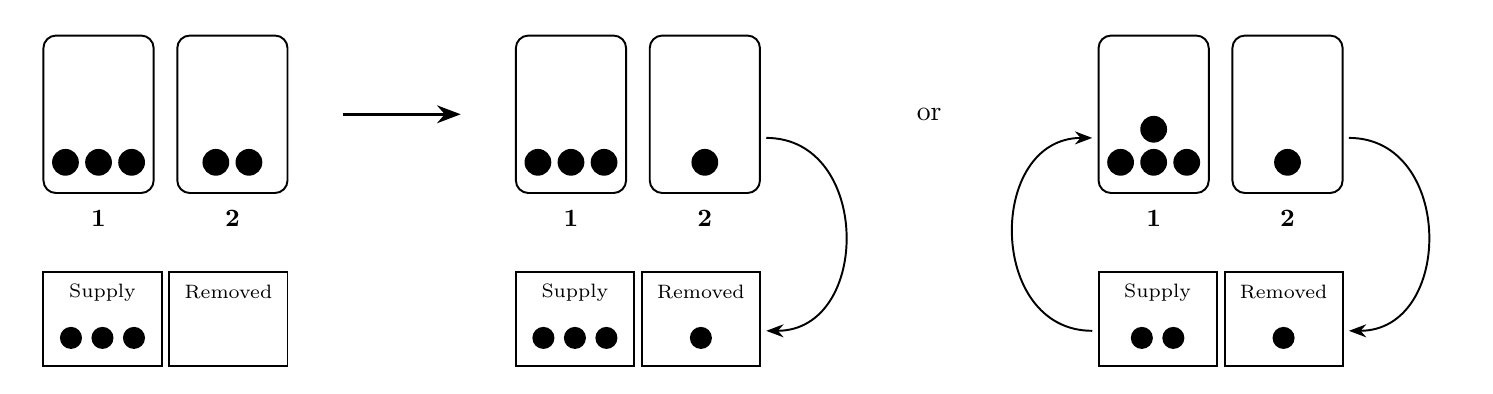
\begin{tikzpicture}[x=1mm,y=1mm]
\useasboundingbox (0,0) rectangle (182.5,43);
\draw[bucket] (2,22) rectangle (16,42);
\node[num] at (9,18.8) {1};
\fill (4.8,25.9) circle (1.7);
\fill (9,25.9) circle (1.7);
\fill (13.2,25.9) circle (1.7);
\draw[bucket] (19,22) rectangle (33,42);
\node[num] at (26,18.8) {2};
\fill (23.9,25.9) circle (1.7);
\fill (28.1,25.9) circle (1.7);
\draw[store] (2,0) rectangle (17,12);
\node[tiny] at (9.5,9.4) {Supply};
\fill (5.5,3.6) circle (1.4);
\fill (9.5,3.6) circle (1.4);
\fill (13.5,3.6) circle (1.4);
\draw[store] (18,0) rectangle (33,12);
\node[tiny] at (25.5,9.4) {Removed};
\draw[bucket] (62,22) rectangle (76,42);
\node[num] at (69,18.8) {1};
\fill (64.8,25.9) circle (1.7);
\fill (69,25.9) circle (1.7);
\fill (73.2,25.9) circle (1.7);
\draw[bucket] (79,22) rectangle (93,42);
\node[num] at (86,18.8) {2};
\fill (86,25.9) circle (1.7);
\draw[store] (62,0) rectangle (77,12);
\node[tiny] at (69.5,9.4) {Supply};
\fill (65.5,3.6) circle (1.4);
\fill (69.5,3.6) circle (1.4);
\fill (73.5,3.6) circle (1.4);
\draw[store] (78,0) rectangle (93,12);
\node[tiny] at (85.5,9.4) {Removed};
\fill (85.5,3.6) circle (1.4);
\draw[flow] (93.8,29) to[out=0,in=0,looseness=1.4] (93.8,4.5);
\draw[bucket] (136,22) rectangle (150,42);
\node[num] at (143,18.8) {1};
\fill (138.8,25.9) circle (1.7);
\fill (143,25.9) circle (1.7);
\fill (147.2,25.9) circle (1.7);
\fill (143,30.1) circle (1.7);
\draw[bucket] (153,22) rectangle (167,42);
\node[num] at (160,18.8) {2};
\fill (160,25.9) circle (1.7);
\draw[store] (136,0) rectangle (151,12);
\node[tiny] at (143.5,9.4) {Supply};
\fill (141.5,3.6) circle (1.4);
\fill (145.5,3.6) circle (1.4);
\draw[store] (152,0) rectangle (167,12);
\node[tiny] at (159.5,9.4) {Removed};
\fill (159.5,3.6) circle (1.4);
\draw[flow] (167.8,29) to[out=0,in=0,looseness=1.4] (167.8,4.5);
\draw[flow] (135.2,4.5) to[out=180,in=180,looseness=1.4] (135.2,29);
\draw[stage] (40,32) -- (55,32);
\node[orword] at (114.5,32) {or};
\end{tikzpicture}\par\vspace{7mm}
\noindent 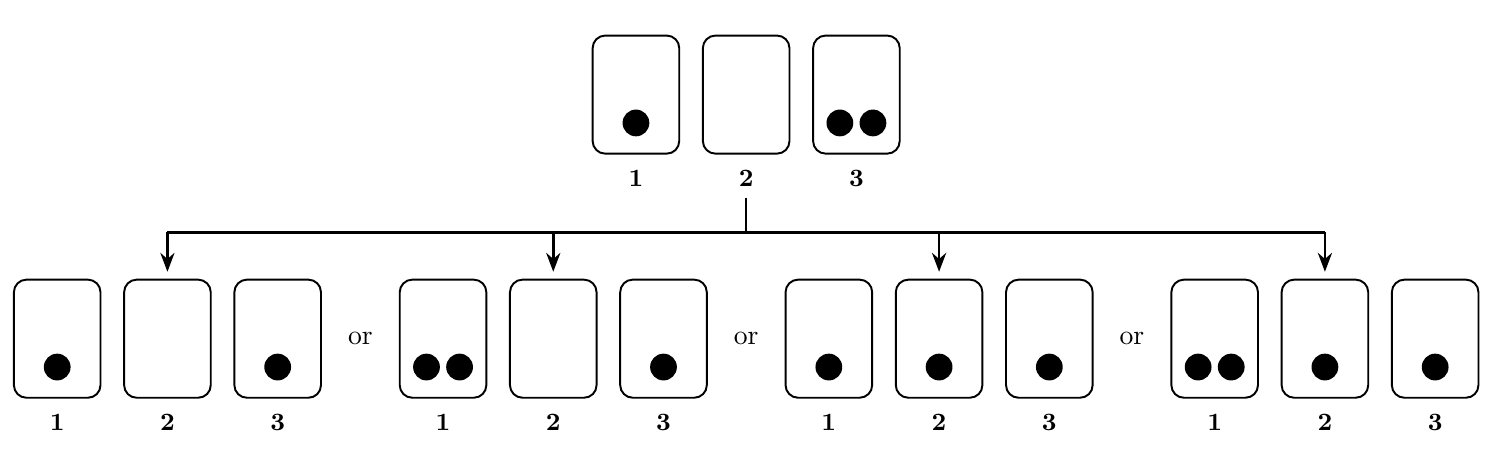
\begin{tikzpicture}[x=1mm,y=1mm]
\useasboundingbox (0,0) rectangle (182.5,52);
\draw[bucket] (71.75,36) rectangle (82.75,51);
\node[num] at (77.25,32.8) {1};
\fill (77.25,39.9) circle (1.7);
\draw[bucket] (85.75,36) rectangle (96.75,51);
\node[num] at (91.25,32.8) {2};
\draw[bucket] (99.75,36) rectangle (110.75,51);
\node[num] at (105.25,32.8) {3};
\fill (103.15,39.9) circle (1.7);
\fill (107.35,39.9) circle (1.7);
\draw[bucket] (-1.75,5) rectangle (9.25,20);
\node[num] at (3.75,1.8) {1};
\fill (3.75,8.9) circle (1.7);
\draw[bucket] (12.25,5) rectangle (23.25,20);
\node[num] at (17.75,1.8) {2};
\draw[bucket] (26.25,5) rectangle (37.25,20);
\node[num] at (31.75,1.8) {3};
\fill (31.75,8.9) circle (1.7);
\node[orword] at (42.25,12.5) {or};
\draw[bucket] (47.25,5) rectangle (58.25,20);
\node[num] at (52.75,1.8) {1};
\fill (50.65,8.9) circle (1.7);
\fill (54.85,8.9) circle (1.7);
\draw[bucket] (61.25,5) rectangle (72.25,20);
\node[num] at (66.75,1.8) {2};
\draw[bucket] (75.25,5) rectangle (86.25,20);
\node[num] at (80.75,1.8) {3};
\fill (80.75,8.9) circle (1.7);
\node[orword] at (91.25,12.5) {or};
\draw[bucket] (96.25,5) rectangle (107.25,20);
\node[num] at (101.75,1.8) {1};
\fill (101.75,8.9) circle (1.7);
\draw[bucket] (110.25,5) rectangle (121.25,20);
\node[num] at (115.75,1.8) {2};
\fill (115.75,8.9) circle (1.7);
\draw[bucket] (124.25,5) rectangle (135.25,20);
\node[num] at (129.75,1.8) {3};
\fill (129.75,8.9) circle (1.7);
\node[orword] at (140.25,12.5) {or};
\draw[bucket] (145.25,5) rectangle (156.25,20);
\node[num] at (150.75,1.8) {1};
\fill (148.65,8.9) circle (1.7);
\fill (152.85,8.9) circle (1.7);
\draw[bucket] (159.25,5) rectangle (170.25,20);
\node[num] at (164.75,1.8) {2};
\fill (164.75,8.9) circle (1.7);
\draw[bucket] (173.25,5) rectangle (184.25,20);
\node[num] at (178.75,1.8) {3};
\fill (178.75,8.9) circle (1.7);
\draw[tree] (91.25,30.4) -- (91.25,26);
\draw[tree] (17.75,26) -- (164.75,26);
\draw[treearrow] (17.75,26) -- (17.75,21);
\draw[treearrow] (66.75,26) -- (66.75,21);
\draw[treearrow] (115.75,26) -- (115.75,21);
\draw[treearrow] (164.75,26) -- (164.75,21);
\end{tikzpicture}\par\vspace{9mm}
\problem{1}{Cover buckets 2 and 3. Put counters in bucket 1 like each picture and play. Circle who wins.}\vspace{5mm}
\noindent 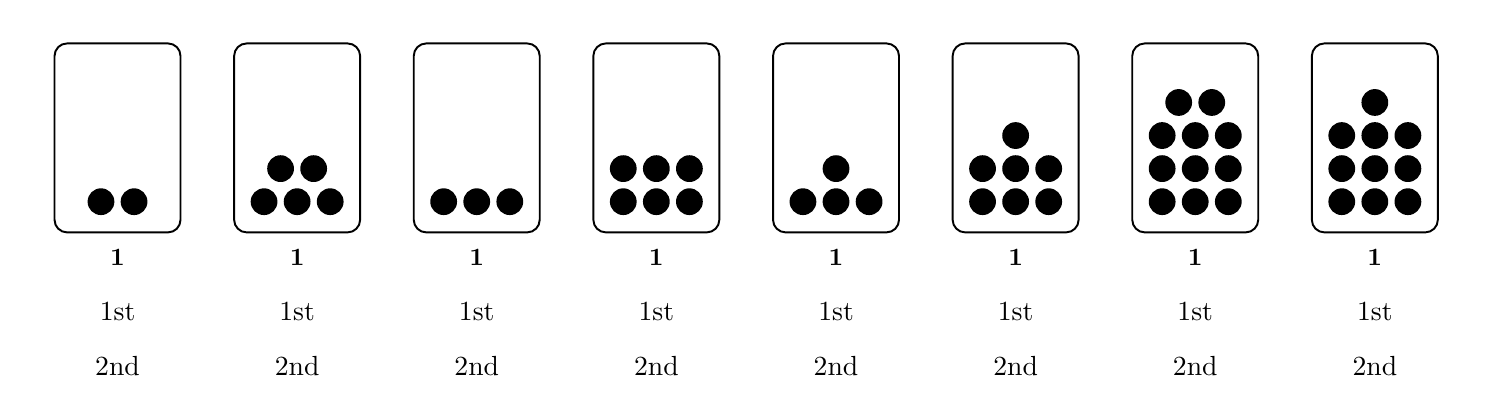
\begin{tikzpicture}[x=1mm,y=1mm]
\useasboundingbox (0,0) rectangle (182.5,46);
\draw[bucket] (3.41,20) rectangle (19.41,44);
\node[num] at (11.41,16.8) {1};
\fill (9.31,23.9) circle (1.7);
\fill (13.51,23.9) circle (1.7);
\node[choice] at (11.41,10) {1st};
\node[choice] at (11.41,3) {2nd};
\draw[bucket] (26.22,20) rectangle (42.22,44);
\node[num] at (34.22,16.8) {1};
\fill (30.02,23.9) circle (1.7);
\fill (34.22,23.9) circle (1.7);
\fill (38.42,23.9) circle (1.7);
\fill (32.12,28.1) circle (1.7);
\fill (36.32,28.1) circle (1.7);
\node[choice] at (34.22,10) {1st};
\node[choice] at (34.22,3) {2nd};
\draw[bucket] (49.03,20) rectangle (65.03,44);
\node[num] at (57.03,16.8) {1};
\fill (52.83,23.9) circle (1.7);
\fill (57.03,23.9) circle (1.7);
\fill (61.23,23.9) circle (1.7);
\node[choice] at (57.03,10) {1st};
\node[choice] at (57.03,3) {2nd};
\draw[bucket] (71.84,20) rectangle (87.84,44);
\node[num] at (79.84,16.8) {1};
\fill (75.64,23.9) circle (1.7);
\fill (79.84,23.9) circle (1.7);
\fill (84.04,23.9) circle (1.7);
\fill (75.64,28.1) circle (1.7);
\fill (79.84,28.1) circle (1.7);
\fill (84.04,28.1) circle (1.7);
\node[choice] at (79.84,10) {1st};
\node[choice] at (79.84,3) {2nd};
\draw[bucket] (94.66,20) rectangle (110.66,44);
\node[num] at (102.66,16.8) {1};
\fill (98.46,23.9) circle (1.7);
\fill (102.66,23.9) circle (1.7);
\fill (106.86,23.9) circle (1.7);
\fill (102.66,28.1) circle (1.7);
\node[choice] at (102.66,10) {1st};
\node[choice] at (102.66,3) {2nd};
\draw[bucket] (117.47,20) rectangle (133.47,44);
\node[num] at (125.47,16.8) {1};
\fill (121.27,23.9) circle (1.7);
\fill (125.47,23.9) circle (1.7);
\fill (129.67,23.9) circle (1.7);
\fill (121.27,28.1) circle (1.7);
\fill (125.47,28.1) circle (1.7);
\fill (129.67,28.1) circle (1.7);
\fill (125.47,32.3) circle (1.7);
\node[choice] at (125.47,10) {1st};
\node[choice] at (125.47,3) {2nd};
\draw[bucket] (140.28,20) rectangle (156.28,44);
\node[num] at (148.28,16.8) {1};
\fill (144.08,23.9) circle (1.7);
\fill (148.28,23.9) circle (1.7);
\fill (152.48,23.9) circle (1.7);
\fill (144.08,28.1) circle (1.7);
\fill (148.28,28.1) circle (1.7);
\fill (152.48,28.1) circle (1.7);
\fill (144.08,32.3) circle (1.7);
\fill (148.28,32.3) circle (1.7);
\fill (152.48,32.3) circle (1.7);
\fill (146.18,36.5) circle (1.7);
\fill (150.38,36.5) circle (1.7);
\node[choice] at (148.28,10) {1st};
\node[choice] at (148.28,3) {2nd};
\draw[bucket] (163.09,20) rectangle (179.09,44);
\node[num] at (171.09,16.8) {1};
\fill (166.89,23.9) circle (1.7);
\fill (171.09,23.9) circle (1.7);
\fill (175.29,23.9) circle (1.7);
\fill (166.89,28.1) circle (1.7);
\fill (171.09,28.1) circle (1.7);
\fill (175.29,28.1) circle (1.7);
\fill (166.89,32.3) circle (1.7);
\fill (171.09,32.3) circle (1.7);
\fill (175.29,32.3) circle (1.7);
\fill (171.09,36.5) circle (1.7);
\node[choice] at (171.09,10) {1st};
\node[choice] at (171.09,3) {2nd};
\end{tikzpicture}\par
\newpage
\problem{2}{Uncover bucket 2. Play from each start, taking turns going first. Circle who can always win.}\vspace{5mm}
\noindent 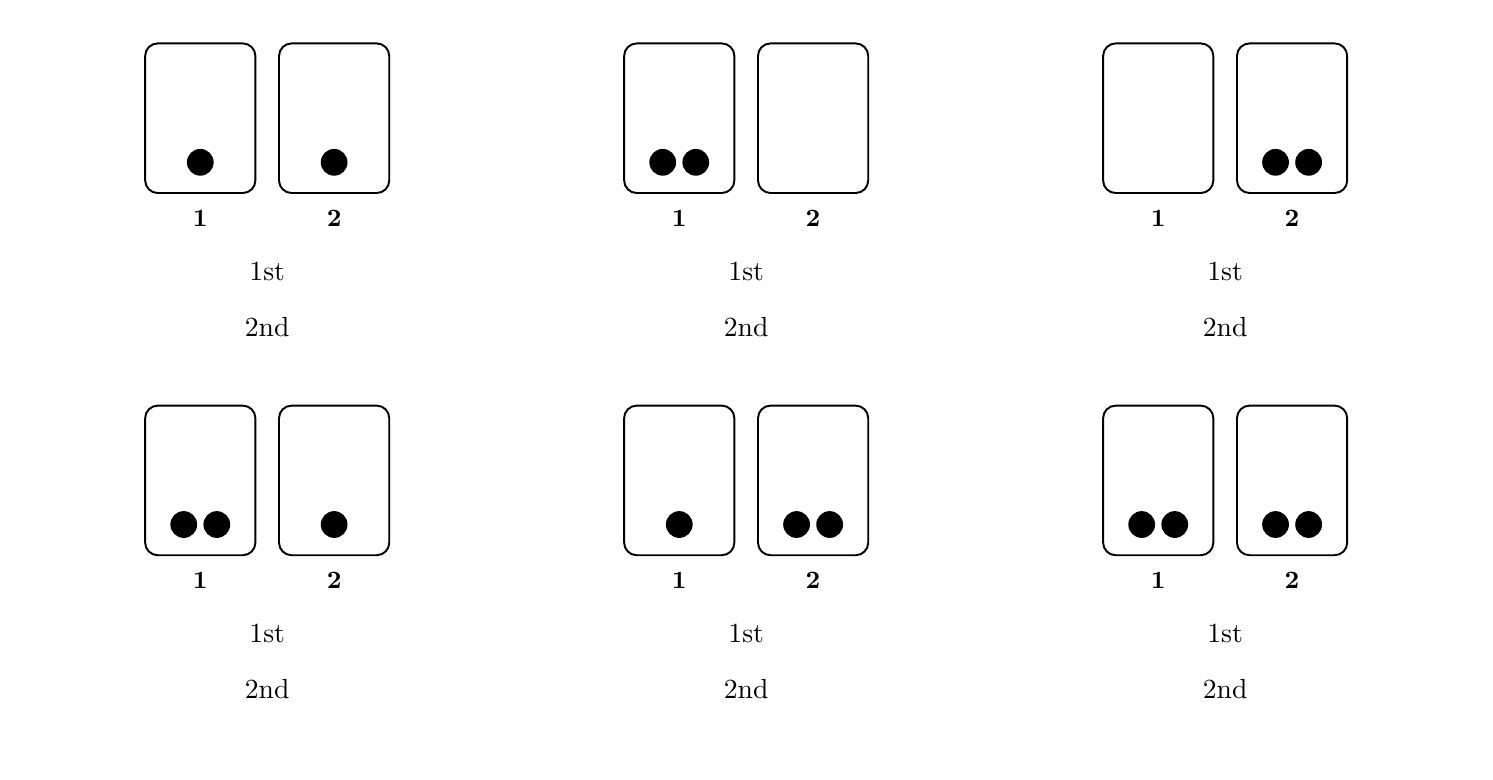
\begin{tikzpicture}[x=1mm,y=1mm]
\useasboundingbox (0,0) rectangle (182.5,92);
\draw[bucket] (14.92,71) rectangle (28.92,90);
\node[num] at (21.92,67.8) {1};
\fill (21.92,74.9) circle (1.7);
\draw[bucket] (31.92,71) rectangle (45.92,90);
\node[num] at (38.92,67.8) {2};
\fill (38.92,74.9) circle (1.7);
\node[choice] at (30.42,61) {1st};
\node[choice] at (30.42,54) {2nd};
\draw[bucket] (75.75,71) rectangle (89.75,90);
\node[num] at (82.75,67.8) {1};
\fill (80.65,74.9) circle (1.7);
\fill (84.85,74.9) circle (1.7);
\draw[bucket] (92.75,71) rectangle (106.75,90);
\node[num] at (99.75,67.8) {2};
\node[choice] at (91.25,61) {1st};
\node[choice] at (91.25,54) {2nd};
\draw[bucket] (136.58,71) rectangle (150.58,90);
\node[num] at (143.58,67.8) {1};
\draw[bucket] (153.58,71) rectangle (167.58,90);
\node[num] at (160.58,67.8) {2};
\fill (158.48,74.9) circle (1.7);
\fill (162.68,74.9) circle (1.7);
\node[choice] at (152.08,61) {1st};
\node[choice] at (152.08,54) {2nd};
\draw[bucket] (14.92,25) rectangle (28.92,44);
\node[num] at (21.92,21.8) {1};
\fill (19.82,28.9) circle (1.7);
\fill (24.02,28.9) circle (1.7);
\draw[bucket] (31.92,25) rectangle (45.92,44);
\node[num] at (38.92,21.8) {2};
\fill (38.92,28.9) circle (1.7);
\node[choice] at (30.42,15) {1st};
\node[choice] at (30.42,8) {2nd};
\draw[bucket] (75.75,25) rectangle (89.75,44);
\node[num] at (82.75,21.8) {1};
\fill (82.75,28.9) circle (1.7);
\draw[bucket] (92.75,25) rectangle (106.75,44);
\node[num] at (99.75,21.8) {2};
\fill (97.65,28.9) circle (1.7);
\fill (101.85,28.9) circle (1.7);
\node[choice] at (91.25,15) {1st};
\node[choice] at (91.25,8) {2nd};
\draw[bucket] (136.58,25) rectangle (150.58,44);
\node[num] at (143.58,21.8) {1};
\fill (141.48,28.9) circle (1.7);
\fill (145.68,28.9) circle (1.7);
\draw[bucket] (153.58,25) rectangle (167.58,44);
\node[num] at (160.58,21.8) {2};
\fill (158.48,28.9) circle (1.7);
\fill (162.68,28.9) circle (1.7);
\node[choice] at (152.08,15) {1st};
\node[choice] at (152.08,8) {2nd};
\end{tikzpicture}\par
\vspace{10mm}
\problem{3}{You go first from each start. Find a first move that lets you always win, and draw the buckets after it.}\vspace{5mm}
\noindent 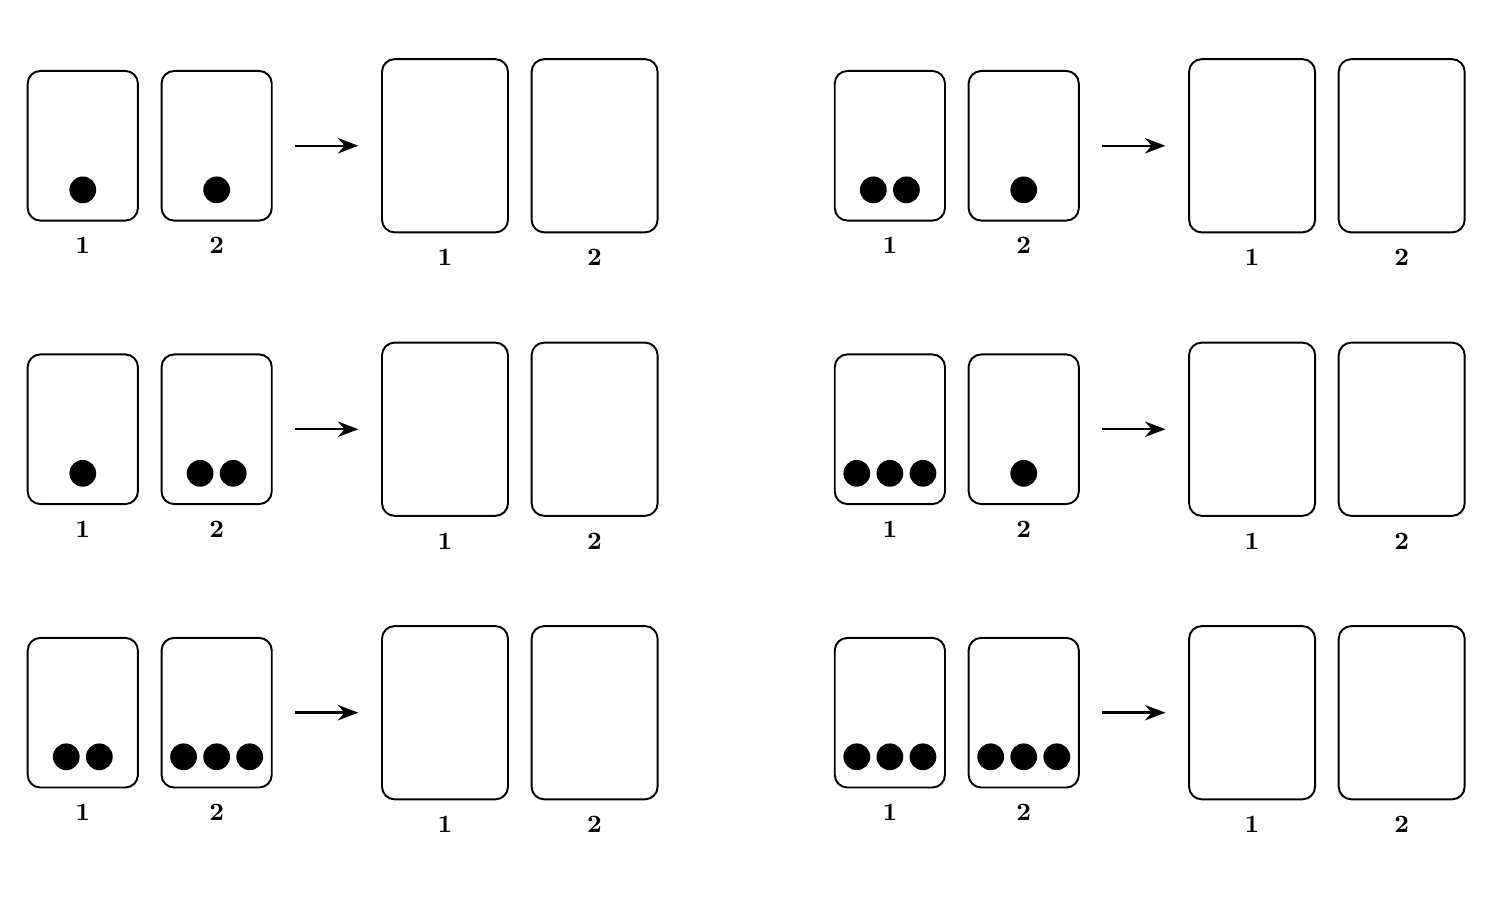
\begin{tikzpicture}[x=1mm,y=1mm]
\useasboundingbox (0,0) rectangle (182.5,108);
\draw[bucket] (0,83.5) rectangle (14,102.5);
\node[num] at (7,80.3) {1};
\fill (7,87.4) circle (1.7);
\draw[bucket] (17,83.5) rectangle (31,102.5);
\node[num] at (24,80.3) {2};
\fill (24,87.4) circle (1.7);
\draw[move] (34,93) -- (42,93);
\draw[bucket] (45,82) rectangle (61,104);
\node[num] at (53,78.8) {1};
\draw[bucket] (64,82) rectangle (80,104);
\node[num] at (72,78.8) {2};
\draw[bucket] (102.5,83.5) rectangle (116.5,102.5);
\node[num] at (109.5,80.3) {1};
\fill (107.4,87.4) circle (1.7);
\fill (111.6,87.4) circle (1.7);
\draw[bucket] (119.5,83.5) rectangle (133.5,102.5);
\node[num] at (126.5,80.3) {2};
\fill (126.5,87.4) circle (1.7);
\draw[move] (136.5,93) -- (144.5,93);
\draw[bucket] (147.5,82) rectangle (163.5,104);
\node[num] at (155.5,78.8) {1};
\draw[bucket] (166.5,82) rectangle (182.5,104);
\node[num] at (174.5,78.8) {2};
\draw[bucket] (0,47.5) rectangle (14,66.5);
\node[num] at (7,44.3) {1};
\fill (7,51.4) circle (1.7);
\draw[bucket] (17,47.5) rectangle (31,66.5);
\node[num] at (24,44.3) {2};
\fill (21.9,51.4) circle (1.7);
\fill (26.1,51.4) circle (1.7);
\draw[move] (34,57) -- (42,57);
\draw[bucket] (45,46) rectangle (61,68);
\node[num] at (53,42.8) {1};
\draw[bucket] (64,46) rectangle (80,68);
\node[num] at (72,42.8) {2};
\draw[bucket] (102.5,47.5) rectangle (116.5,66.5);
\node[num] at (109.5,44.3) {1};
\fill (105.3,51.4) circle (1.7);
\fill (109.5,51.4) circle (1.7);
\fill (113.7,51.4) circle (1.7);
\draw[bucket] (119.5,47.5) rectangle (133.5,66.5);
\node[num] at (126.5,44.3) {2};
\fill (126.5,51.4) circle (1.7);
\draw[move] (136.5,57) -- (144.5,57);
\draw[bucket] (147.5,46) rectangle (163.5,68);
\node[num] at (155.5,42.8) {1};
\draw[bucket] (166.5,46) rectangle (182.5,68);
\node[num] at (174.5,42.8) {2};
\draw[bucket] (0,11.5) rectangle (14,30.5);
\node[num] at (7,8.3) {1};
\fill (4.9,15.4) circle (1.7);
\fill (9.1,15.4) circle (1.7);
\draw[bucket] (17,11.5) rectangle (31,30.5);
\node[num] at (24,8.3) {2};
\fill (19.8,15.4) circle (1.7);
\fill (24,15.4) circle (1.7);
\fill (28.2,15.4) circle (1.7);
\draw[move] (34,21) -- (42,21);
\draw[bucket] (45,10) rectangle (61,32);
\node[num] at (53,6.8) {1};
\draw[bucket] (64,10) rectangle (80,32);
\node[num] at (72,6.8) {2};
\draw[bucket] (102.5,11.5) rectangle (116.5,30.5);
\node[num] at (109.5,8.3) {1};
\fill (105.3,15.4) circle (1.7);
\fill (109.5,15.4) circle (1.7);
\fill (113.7,15.4) circle (1.7);
\draw[bucket] (119.5,11.5) rectangle (133.5,30.5);
\node[num] at (126.5,8.3) {2};
\fill (122.3,15.4) circle (1.7);
\fill (126.5,15.4) circle (1.7);
\fill (130.7,15.4) circle (1.7);
\draw[move] (136.5,21) -- (144.5,21);
\draw[bucket] (147.5,10) rectangle (163.5,32);
\node[num] at (155.5,6.8) {1};
\draw[bucket] (166.5,10) rectangle (182.5,32);
\node[num] at (174.5,6.8) {2};
\end{tikzpicture}\par
\newpage
\problem{4}{Play against the adult from each start, taking turns going first. Circle who can always win, and show the adult how.}\vspace{5mm}
\noindent 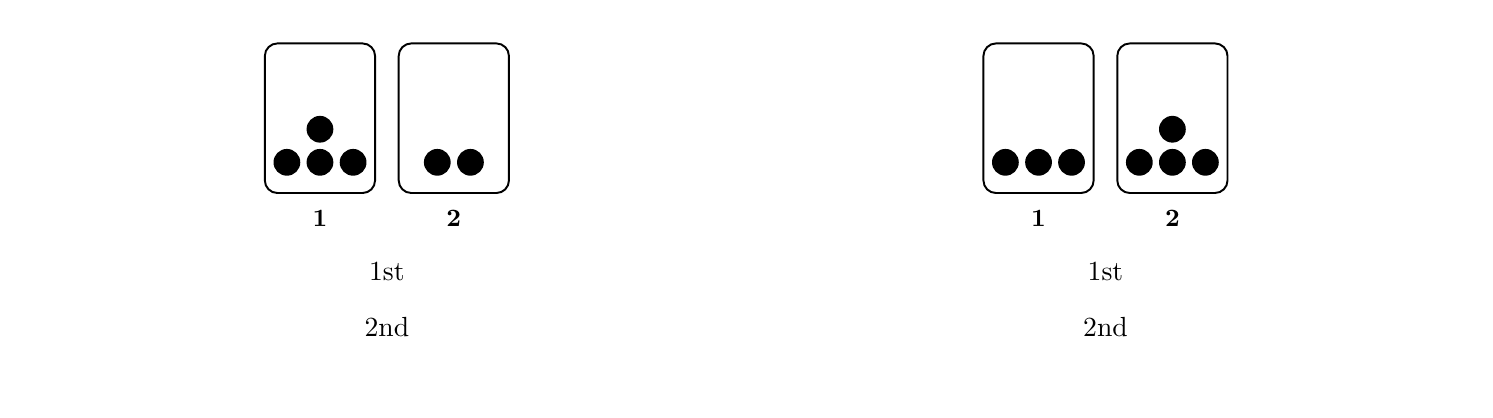
\begin{tikzpicture}[x=1mm,y=1mm]
\useasboundingbox (0,0) rectangle (182.5,46);
\draw[bucket] (30.12,25) rectangle (44.12,44);
\node[num] at (37.12,21.8) {1};
\fill (32.92,28.9) circle (1.7);
\fill (37.12,28.9) circle (1.7);
\fill (41.33,28.9) circle (1.7);
\fill (37.12,33.1) circle (1.7);
\draw[bucket] (47.12,25) rectangle (61.12,44);
\node[num] at (54.12,21.8) {2};
\fill (52.02,28.9) circle (1.7);
\fill (56.23,28.9) circle (1.7);
\node[choice] at (45.62,15) {1st};
\node[choice] at (45.62,8) {2nd};
\draw[bucket] (121.38,25) rectangle (135.38,44);
\node[num] at (128.38,21.8) {1};
\fill (124.17,28.9) circle (1.7);
\fill (128.38,28.9) circle (1.7);
\fill (132.57,28.9) circle (1.7);
\draw[bucket] (138.38,25) rectangle (152.38,44);
\node[num] at (145.38,21.8) {2};
\fill (141.18,28.9) circle (1.7);
\fill (145.38,28.9) circle (1.7);
\fill (149.57,28.9) circle (1.7);
\fill (145.38,33.1) circle (1.7);
\node[choice] at (136.88,15) {1st};
\node[choice] at (136.88,8) {2nd};
\end{tikzpicture}\par
\vspace{10mm}
\problem{5}{Your partner goes first from this start. Draw the buckets after each move your partner can make. Next to each, draw the buckets after a move that lets you always win.}\vspace{5mm}
\noindent 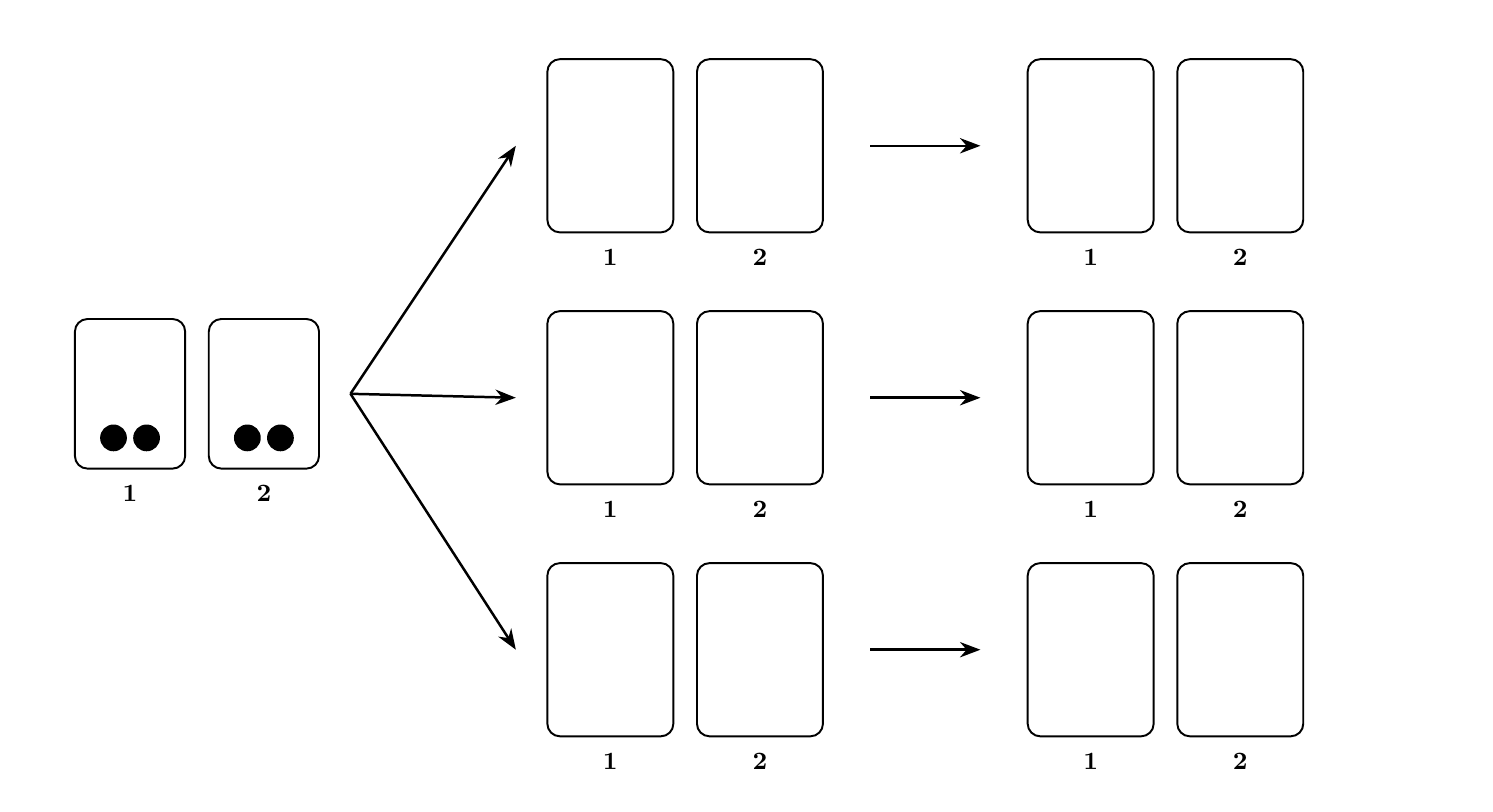
\begin{tikzpicture}[x=1mm,y=1mm]
\useasboundingbox (0,0) rectangle (182.5,96);
\draw[bucket] (6,40) rectangle (20,59);
\node[num] at (13,36.8) {1};
\fill (10.9,43.9) circle (1.7);
\fill (15.1,43.9) circle (1.7);
\draw[bucket] (23,40) rectangle (37,59);
\node[num] at (30,36.8) {2};
\fill (27.9,43.9) circle (1.7);
\fill (32.1,43.9) circle (1.7);
\draw[move] (41,49.5) -- (62,81);
\draw[bucket] (66,70) rectangle (82,92);
\node[num] at (74,66.8) {1};
\draw[bucket] (85,70) rectangle (101,92);
\node[num] at (93,66.8) {2};
\draw[move] (107,81) -- (121,81);
\draw[bucket] (127,70) rectangle (143,92);
\node[num] at (135,66.8) {1};
\draw[bucket] (146,70) rectangle (162,92);
\node[num] at (154,66.8) {2};
\draw[move] (41,49.5) -- (62,49);
\draw[bucket] (66,38) rectangle (82,60);
\node[num] at (74,34.8) {1};
\draw[bucket] (85,38) rectangle (101,60);
\node[num] at (93,34.8) {2};
\draw[move] (107,49) -- (121,49);
\draw[bucket] (127,38) rectangle (143,60);
\node[num] at (135,34.8) {1};
\draw[bucket] (146,38) rectangle (162,60);
\node[num] at (154,34.8) {2};
\draw[move] (41,49.5) -- (62,17);
\draw[bucket] (66,6) rectangle (82,28);
\node[num] at (74,2.8) {1};
\draw[bucket] (85,6) rectangle (101,28);
\node[num] at (93,2.8) {2};
\draw[move] (107,17) -- (121,17);
\draw[bucket] (127,6) rectangle (143,28);
\node[num] at (135,2.8) {1};
\draw[bucket] (146,6) rectangle (162,28);
\node[num] at (154,2.8) {2};
\end{tikzpicture}\par
\newpage
\problem{6}{Find every way to put 4 counters into buckets 1 and 2 so that the player who goes second can always win. A bucket can be empty. Then do the same with 6 counters.}\vspace{5mm}
\noindent 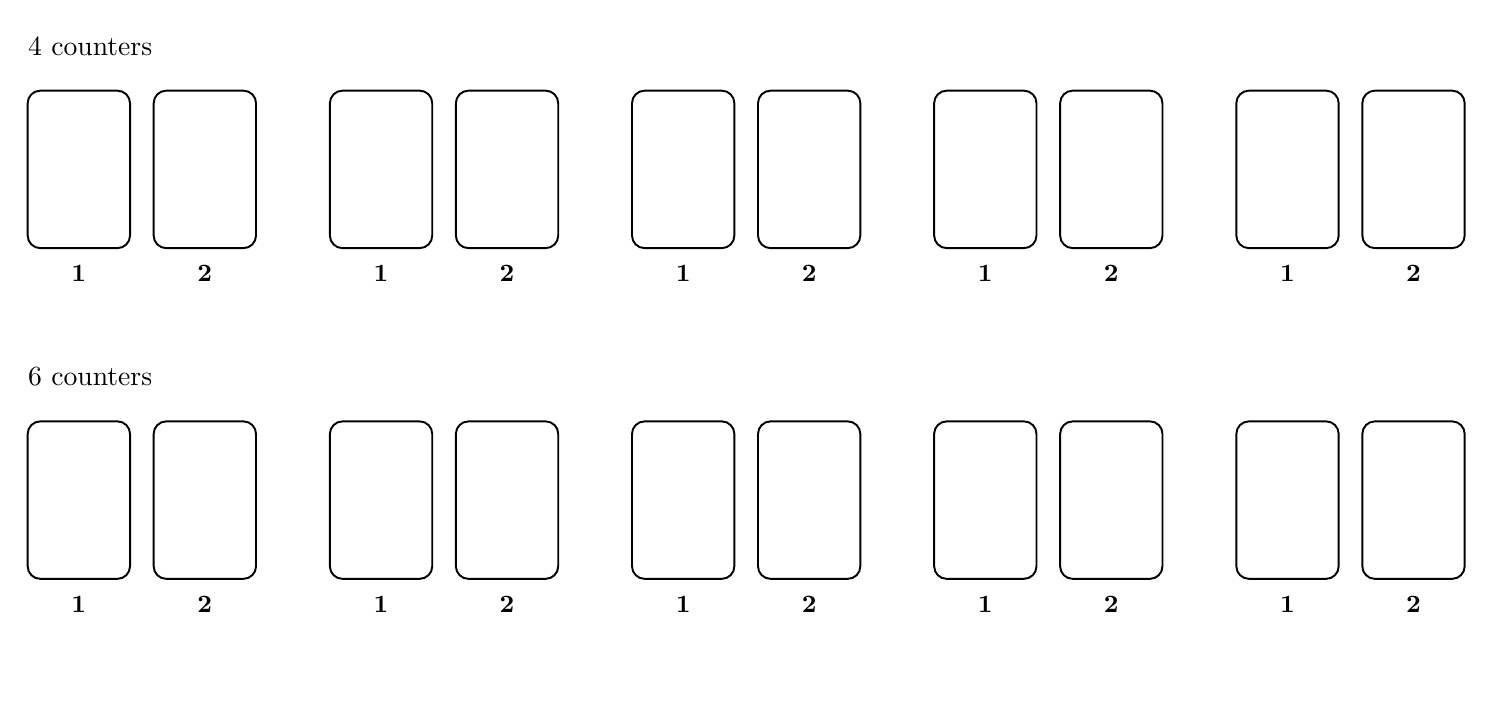
\begin{tikzpicture}[x=1mm,y=1mm]
\useasboundingbox (0,0) rectangle (182.5,84);
\node[rowlab,anchor=north west,inner xsep=0] at (0,84) {4 counters};
\draw[bucket] (0,56) rectangle (13,76);
\node[num] at (6.5,52.8) {1};
\draw[bucket] (16,56) rectangle (29,76);
\node[num] at (22.5,52.8) {2};
\draw[bucket] (38.38,56) rectangle (51.38,76);
\node[num] at (44.88,52.8) {1};
\draw[bucket] (54.38,56) rectangle (67.38,76);
\node[num] at (60.88,52.8) {2};
\draw[bucket] (76.75,56) rectangle (89.75,76);
\node[num] at (83.25,52.8) {1};
\draw[bucket] (92.75,56) rectangle (105.75,76);
\node[num] at (99.25,52.8) {2};
\draw[bucket] (115.12,56) rectangle (128.12,76);
\node[num] at (121.62,52.8) {1};
\draw[bucket] (131.12,56) rectangle (144.12,76);
\node[num] at (137.62,52.8) {2};
\draw[bucket] (153.5,56) rectangle (166.5,76);
\node[num] at (160,52.8) {1};
\draw[bucket] (169.5,56) rectangle (182.5,76);
\node[num] at (176,52.8) {2};
\node[rowlab,anchor=north west,inner xsep=0] at (0,42) {6 counters};
\draw[bucket] (0,14) rectangle (13,34);
\node[num] at (6.5,10.8) {1};
\draw[bucket] (16,14) rectangle (29,34);
\node[num] at (22.5,10.8) {2};
\draw[bucket] (38.38,14) rectangle (51.38,34);
\node[num] at (44.88,10.8) {1};
\draw[bucket] (54.38,14) rectangle (67.38,34);
\node[num] at (60.88,10.8) {2};
\draw[bucket] (76.75,14) rectangle (89.75,34);
\node[num] at (83.25,10.8) {1};
\draw[bucket] (92.75,14) rectangle (105.75,34);
\node[num] at (99.25,10.8) {2};
\draw[bucket] (115.12,14) rectangle (128.12,34);
\node[num] at (121.62,10.8) {1};
\draw[bucket] (131.12,14) rectangle (144.12,34);
\node[num] at (137.62,10.8) {2};
\draw[bucket] (153.5,14) rectangle (166.5,34);
\node[num] at (160,10.8) {1};
\draw[bucket] (169.5,14) rectangle (182.5,34);
\node[num] at (176,10.8) {2};
\end{tikzpicture}\par
\vspace{10mm}
\problem{7}{If you can, put 5 counters into buckets 1 and 2 so that the player who goes second can always win. If you can't, explain why.}\vspace{5mm}
\noindent \begin{tikzpicture}[x=1mm,y=1mm]
\useasboundingbox (0,0) rectangle (182.5,30);
\draw[bucket] (6,6) rectangle (22,28);
\node[num] at (14,2.8) {1};
\draw[bucket] (25,6) rectangle (41,28);
\node[num] at (33,2.8) {2};
\end{tikzpicture}\par
\newpage
\problem{8}{Work together. From each start, make the game as short as you can and then as long as you can. Write how many counters end up in Removed.}\vspace{5mm}
\noindent 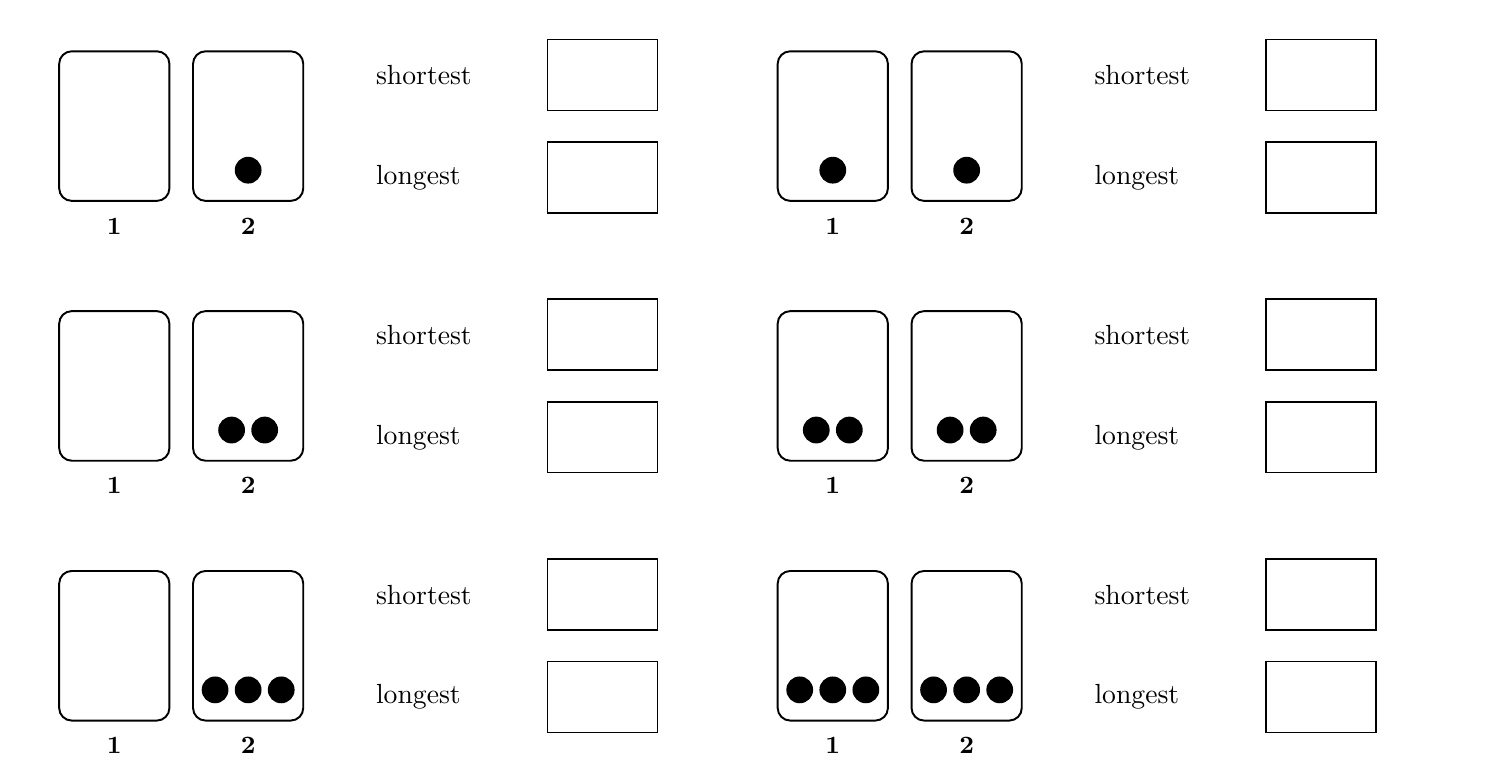
\begin{tikzpicture}[x=1mm,y=1mm]
\useasboundingbox (0,0) rectangle (182.5,92);
\draw[bucket] (4,70) rectangle (18,89);
\node[num] at (11,66.8) {1};
\draw[bucket] (21,70) rectangle (35,89);
\node[num] at (28,66.8) {2};
\fill (28,73.9) circle (1.7);
\node[choice,anchor=west] at (43,86) {shortest};
\node[choice,anchor=west] at (43,73) {longest};
\draw[ans] (66,81.5) rectangle (80,90.5);
\draw[ans] (66,68.5) rectangle (80,77.5);
\draw[bucket] (4,37) rectangle (18,56);
\node[num] at (11,33.8) {1};
\draw[bucket] (21,37) rectangle (35,56);
\node[num] at (28,33.8) {2};
\fill (25.9,40.9) circle (1.7);
\fill (30.1,40.9) circle (1.7);
\node[choice,anchor=west] at (43,53) {shortest};
\node[choice,anchor=west] at (43,40) {longest};
\draw[ans] (66,48.5) rectangle (80,57.5);
\draw[ans] (66,35.5) rectangle (80,44.5);
\draw[bucket] (4,4) rectangle (18,23);
\node[num] at (11,0.8) {1};
\draw[bucket] (21,4) rectangle (35,23);
\node[num] at (28,0.8) {2};
\fill (23.8,7.9) circle (1.7);
\fill (28,7.9) circle (1.7);
\fill (32.2,7.9) circle (1.7);
\node[choice,anchor=west] at (43,20) {shortest};
\node[choice,anchor=west] at (43,7) {longest};
\draw[ans] (66,15.5) rectangle (80,24.5);
\draw[ans] (66,2.5) rectangle (80,11.5);
\draw[bucket] (95.25,70) rectangle (109.25,89);
\node[num] at (102.25,66.8) {1};
\fill (102.25,73.9) circle (1.7);
\draw[bucket] (112.25,70) rectangle (126.25,89);
\node[num] at (119.25,66.8) {2};
\fill (119.25,73.9) circle (1.7);
\node[choice,anchor=west] at (134.25,86) {shortest};
\node[choice,anchor=west] at (134.25,73) {longest};
\draw[ans] (157.25,81.5) rectangle (171.25,90.5);
\draw[ans] (157.25,68.5) rectangle (171.25,77.5);
\draw[bucket] (95.25,37) rectangle (109.25,56);
\node[num] at (102.25,33.8) {1};
\fill (100.15,40.9) circle (1.7);
\fill (104.35,40.9) circle (1.7);
\draw[bucket] (112.25,37) rectangle (126.25,56);
\node[num] at (119.25,33.8) {2};
\fill (117.15,40.9) circle (1.7);
\fill (121.35,40.9) circle (1.7);
\node[choice,anchor=west] at (134.25,53) {shortest};
\node[choice,anchor=west] at (134.25,40) {longest};
\draw[ans] (157.25,48.5) rectangle (171.25,57.5);
\draw[ans] (157.25,35.5) rectangle (171.25,44.5);
\draw[bucket] (95.25,4) rectangle (109.25,23);
\node[num] at (102.25,0.8) {1};
\fill (98.05,7.9) circle (1.7);
\fill (102.25,7.9) circle (1.7);
\fill (106.45,7.9) circle (1.7);
\draw[bucket] (112.25,4) rectangle (126.25,23);
\node[num] at (119.25,0.8) {2};
\fill (115.05,7.9) circle (1.7);
\fill (119.25,7.9) circle (1.7);
\fill (123.45,7.9) circle (1.7);
\node[choice,anchor=west] at (134.25,20) {shortest};
\node[choice,anchor=west] at (134.25,7) {longest};
\draw[ans] (157.25,15.5) rectangle (171.25,24.5);
\draw[ans] (157.25,2.5) rectangle (171.25,11.5);
\end{tikzpicture}\par
\vspace{10mm}
\problem{9}{Uncover bucket 3. Work together to make the buckets hold as many counters as you can. Write the most they hold.}\vspace{5mm}
\noindent 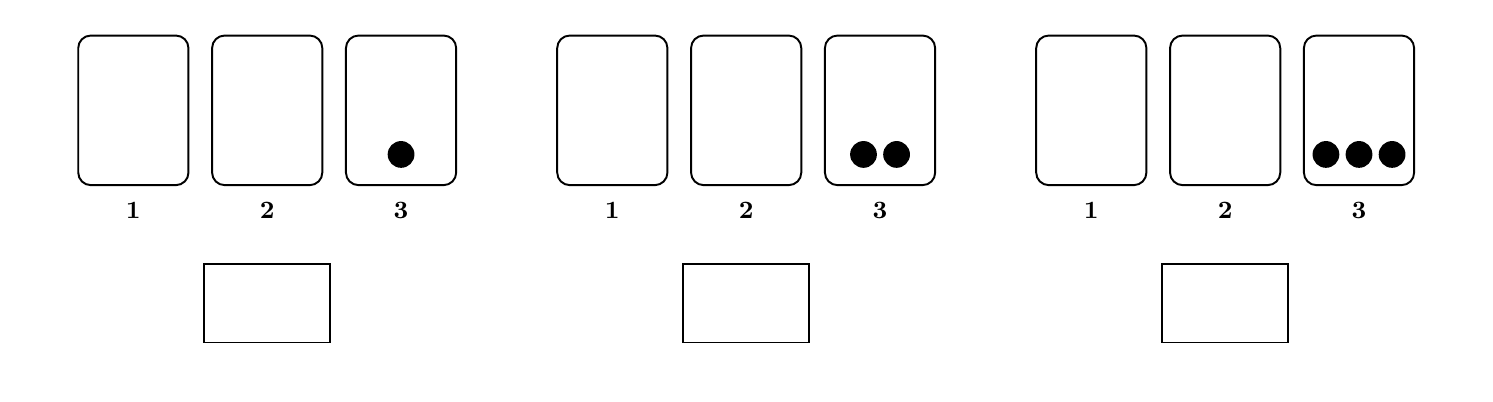
\begin{tikzpicture}[x=1mm,y=1mm]
\useasboundingbox (0,0) rectangle (182.5,44);
\draw[bucket] (6.42,24) rectangle (20.42,43);
\node[num] at (13.42,20.8) {1};
\draw[bucket] (23.42,24) rectangle (37.42,43);
\node[num] at (30.42,20.8) {2};
\draw[bucket] (40.42,24) rectangle (54.42,43);
\node[num] at (47.42,20.8) {3};
\fill (47.42,27.9) circle (1.7);
\draw[ans] (22.42,4) rectangle (38.42,14);
\draw[bucket] (67.25,24) rectangle (81.25,43);
\node[num] at (74.25,20.8) {1};
\draw[bucket] (84.25,24) rectangle (98.25,43);
\node[num] at (91.25,20.8) {2};
\draw[bucket] (101.25,24) rectangle (115.25,43);
\node[num] at (108.25,20.8) {3};
\fill (106.15,27.9) circle (1.7);
\fill (110.35,27.9) circle (1.7);
\draw[ans] (83.25,4) rectangle (99.25,14);
\draw[bucket] (128.08,24) rectangle (142.08,43);
\node[num] at (135.08,20.8) {1};
\draw[bucket] (145.08,24) rectangle (159.08,43);
\node[num] at (152.08,20.8) {2};
\draw[bucket] (162.08,24) rectangle (176.08,43);
\node[num] at (169.08,20.8) {3};
\fill (164.88,27.9) circle (1.7);
\fill (169.08,27.9) circle (1.7);
\fill (173.28,27.9) circle (1.7);
\draw[ans] (144.08,4) rectangle (160.08,14);
\end{tikzpicture}\par
\newpage
\problem{10}{You go first from each start. Find a first move that lets you always win, and draw the buckets after it.}\vspace{5mm}
\noindent 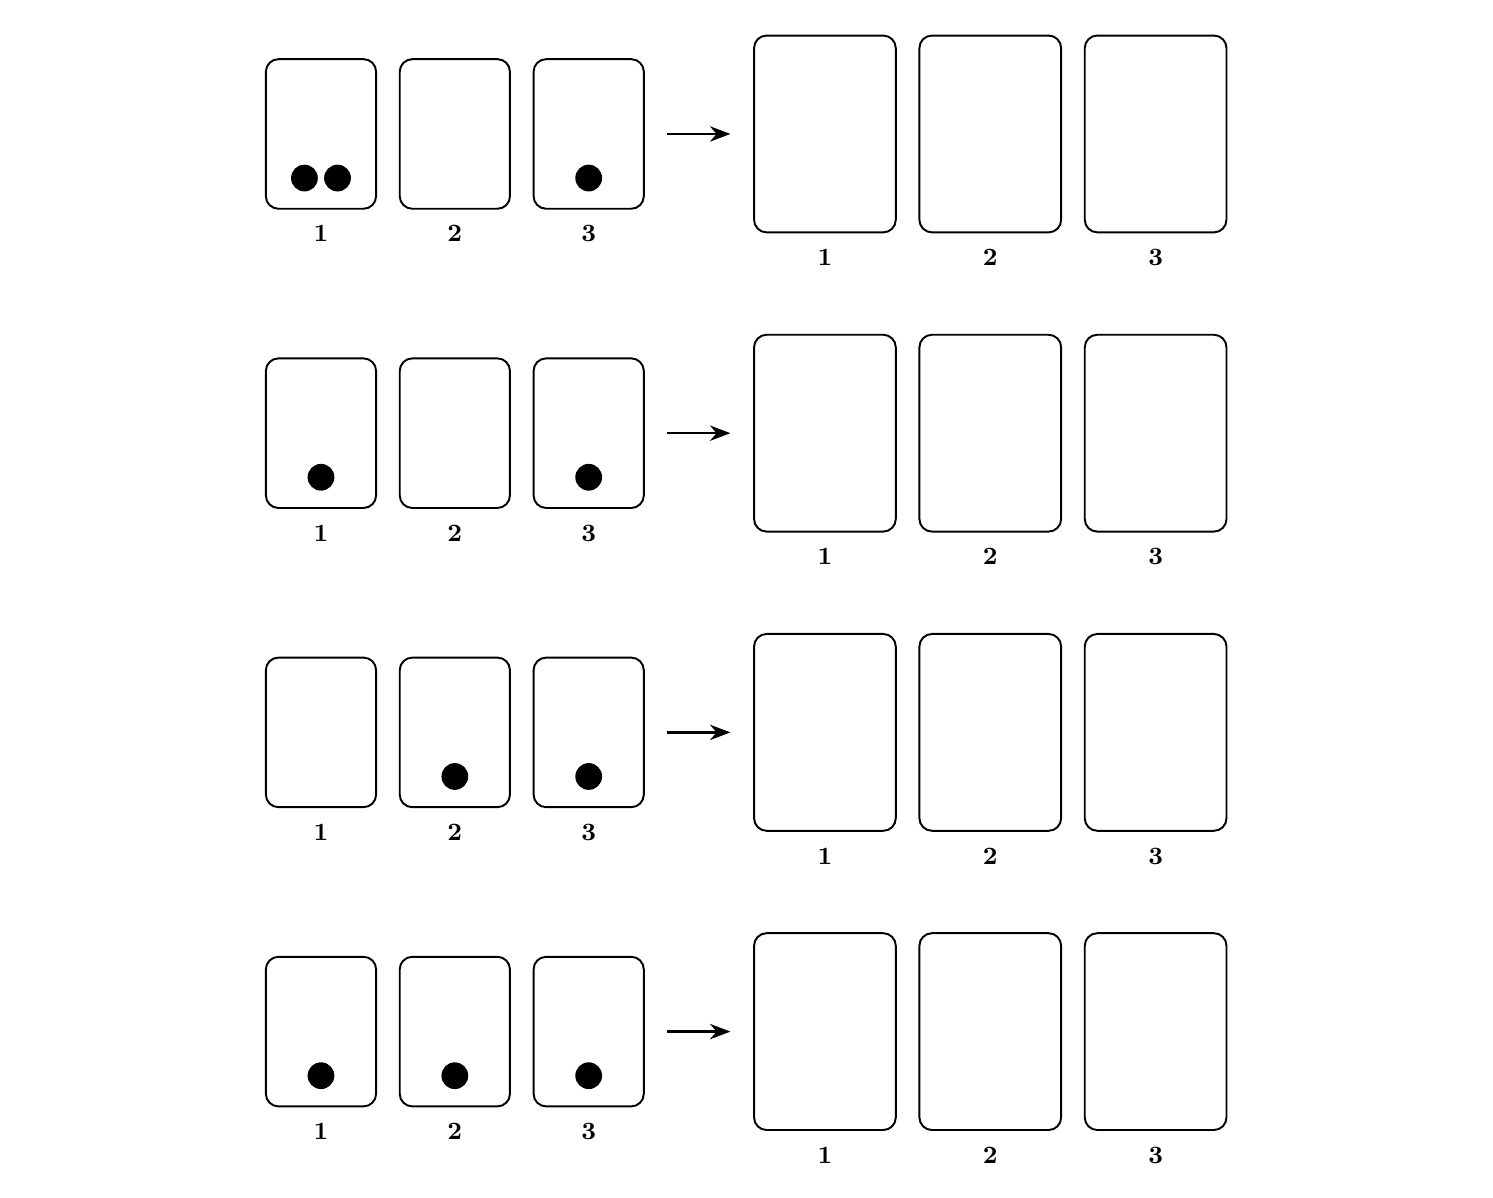
\begin{tikzpicture}[x=1mm,y=1mm]
\useasboundingbox (0,0) rectangle (182.5,145);
\draw[bucket] (30.25,122) rectangle (44.25,141);
\node[num] at (37.25,118.8) {1};
\fill (35.15,125.9) circle (1.7);
\fill (39.35,125.9) circle (1.7);
\draw[bucket] (47.25,122) rectangle (61.25,141);
\node[num] at (54.25,118.8) {2};
\draw[bucket] (64.25,122) rectangle (78.25,141);
\node[num] at (71.25,118.8) {3};
\fill (71.25,125.9) circle (1.7);
\draw[move] (81.25,131.5) -- (89.25,131.5);
\draw[bucket] (92.25,119) rectangle (110.25,144);
\node[num] at (101.25,115.8) {1};
\draw[bucket] (113.25,119) rectangle (131.25,144);
\node[num] at (122.25,115.8) {2};
\draw[bucket] (134.25,119) rectangle (152.25,144);
\node[num] at (143.25,115.8) {3};
\draw[bucket] (30.25,84) rectangle (44.25,103);
\node[num] at (37.25,80.8) {1};
\fill (37.25,87.9) circle (1.7);
\draw[bucket] (47.25,84) rectangle (61.25,103);
\node[num] at (54.25,80.8) {2};
\draw[bucket] (64.25,84) rectangle (78.25,103);
\node[num] at (71.25,80.8) {3};
\fill (71.25,87.9) circle (1.7);
\draw[move] (81.25,93.5) -- (89.25,93.5);
\draw[bucket] (92.25,81) rectangle (110.25,106);
\node[num] at (101.25,77.8) {1};
\draw[bucket] (113.25,81) rectangle (131.25,106);
\node[num] at (122.25,77.8) {2};
\draw[bucket] (134.25,81) rectangle (152.25,106);
\node[num] at (143.25,77.8) {3};
\draw[bucket] (30.25,46) rectangle (44.25,65);
\node[num] at (37.25,42.8) {1};
\draw[bucket] (47.25,46) rectangle (61.25,65);
\node[num] at (54.25,42.8) {2};
\fill (54.25,49.9) circle (1.7);
\draw[bucket] (64.25,46) rectangle (78.25,65);
\node[num] at (71.25,42.8) {3};
\fill (71.25,49.9) circle (1.7);
\draw[move] (81.25,55.5) -- (89.25,55.5);
\draw[bucket] (92.25,43) rectangle (110.25,68);
\node[num] at (101.25,39.8) {1};
\draw[bucket] (113.25,43) rectangle (131.25,68);
\node[num] at (122.25,39.8) {2};
\draw[bucket] (134.25,43) rectangle (152.25,68);
\node[num] at (143.25,39.8) {3};
\draw[bucket] (30.25,8) rectangle (44.25,27);
\node[num] at (37.25,4.8) {1};
\fill (37.25,11.9) circle (1.7);
\draw[bucket] (47.25,8) rectangle (61.25,27);
\node[num] at (54.25,4.8) {2};
\fill (54.25,11.9) circle (1.7);
\draw[bucket] (64.25,8) rectangle (78.25,27);
\node[num] at (71.25,4.8) {3};
\fill (71.25,11.9) circle (1.7);
\draw[move] (81.25,17.5) -- (89.25,17.5);
\draw[bucket] (92.25,5) rectangle (110.25,30);
\node[num] at (101.25,1.8) {1};
\draw[bucket] (113.25,5) rectangle (131.25,30);
\node[num] at (122.25,1.8) {2};
\draw[bucket] (134.25,5) rectangle (152.25,30);
\node[num] at (143.25,1.8) {3};
\end{tikzpicture}\par
\newpage
\problem{11}{Work together to make the game from each start last as long as you can. Write how many counters end up in Removed.}\vspace{5mm}
\noindent 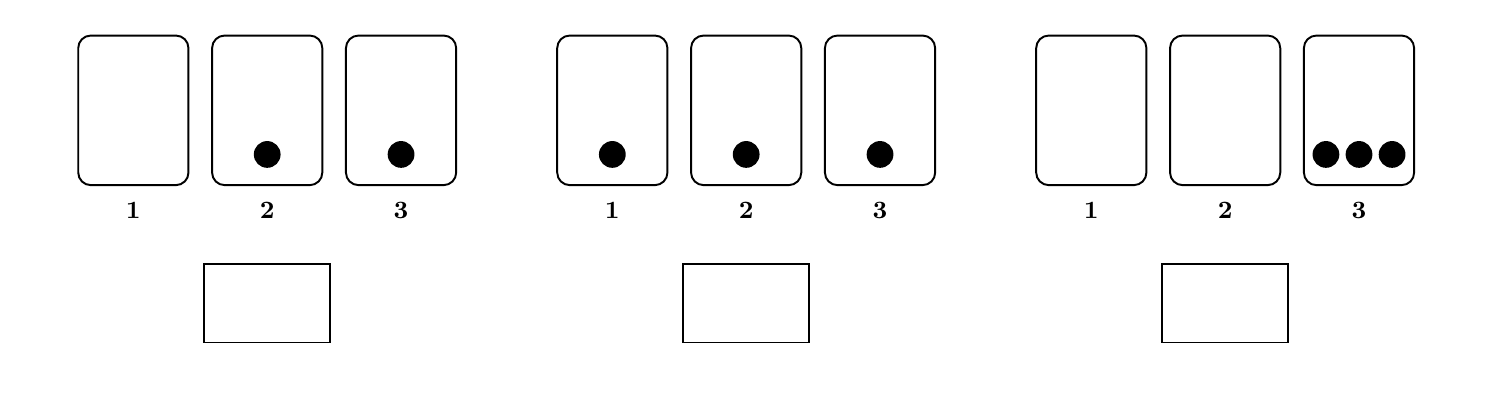
\begin{tikzpicture}[x=1mm,y=1mm]
\useasboundingbox (0,0) rectangle (182.5,44);
\draw[bucket] (6.42,24) rectangle (20.42,43);
\node[num] at (13.42,20.8) {1};
\draw[bucket] (23.42,24) rectangle (37.42,43);
\node[num] at (30.42,20.8) {2};
\fill (30.42,27.9) circle (1.7);
\draw[bucket] (40.42,24) rectangle (54.42,43);
\node[num] at (47.42,20.8) {3};
\fill (47.42,27.9) circle (1.7);
\draw[ans] (22.42,4) rectangle (38.42,14);
\draw[bucket] (67.25,24) rectangle (81.25,43);
\node[num] at (74.25,20.8) {1};
\fill (74.25,27.9) circle (1.7);
\draw[bucket] (84.25,24) rectangle (98.25,43);
\node[num] at (91.25,20.8) {2};
\fill (91.25,27.9) circle (1.7);
\draw[bucket] (101.25,24) rectangle (115.25,43);
\node[num] at (108.25,20.8) {3};
\fill (108.25,27.9) circle (1.7);
\draw[ans] (83.25,4) rectangle (99.25,14);
\draw[bucket] (128.08,24) rectangle (142.08,43);
\node[num] at (135.08,20.8) {1};
\draw[bucket] (145.08,24) rectangle (159.08,43);
\node[num] at (152.08,20.8) {2};
\draw[bucket] (162.08,24) rectangle (176.08,43);
\node[num] at (169.08,20.8) {3};
\fill (164.88,27.9) circle (1.7);
\fill (169.08,27.9) circle (1.7);
\fill (173.28,27.9) circle (1.7);
\draw[ans] (144.08,4) rectangle (160.08,14);
\end{tikzpicture}\par
\vspace{10mm}
\problem{12}{Could a game from this start go on forever? Explain.}\vspace{5mm}
\noindent 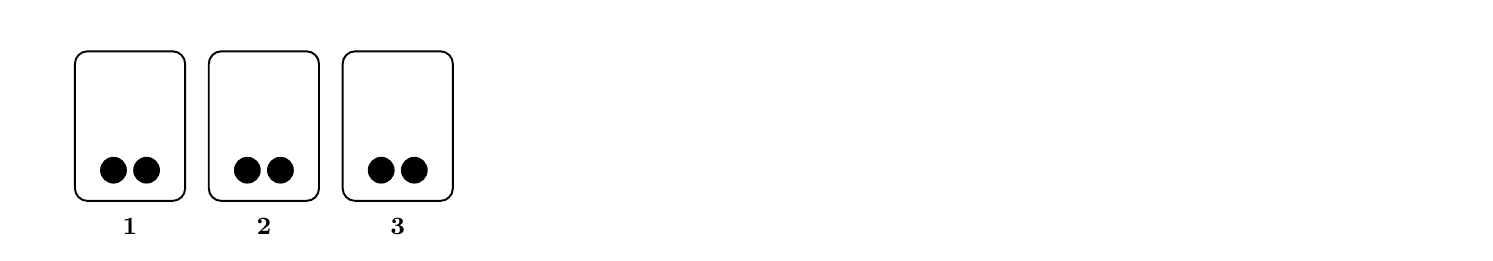
\begin{tikzpicture}[x=1mm,y=1mm]
\useasboundingbox (0,0) rectangle (182.5,26);
\draw[bucket] (6,4) rectangle (20,23);
\node[num] at (13,0.8) {1};
\fill (10.9,7.9) circle (1.7);
\fill (15.1,7.9) circle (1.7);
\draw[bucket] (23,4) rectangle (37,23);
\node[num] at (30,0.8) {2};
\fill (27.9,7.9) circle (1.7);
\fill (32.1,7.9) circle (1.7);
\draw[bucket] (40,4) rectangle (54,23);
\node[num] at (47,0.8) {3};
\fill (44.9,7.9) circle (1.7);
\fill (49.1,7.9) circle (1.7);
\end{tikzpicture}\par
\end{document}
